\section{Problem definition}

In this project, the structure of a parachute is going to be analyzed in order
to obtain the strain and stress of each one of his elements under typical
operation in flight, considering the mass of the system and the drag forces
due to the air.\\

The structure of the parachute to be studied is shown in the figure \ref{fig:definition},
where it's also indicated the types and structure of the materials used for the
bars. This will be of two different types of material, named as "\textit{bars}" and
"\textit{cables}".\\

\begin{figure}[h]
	\centering
	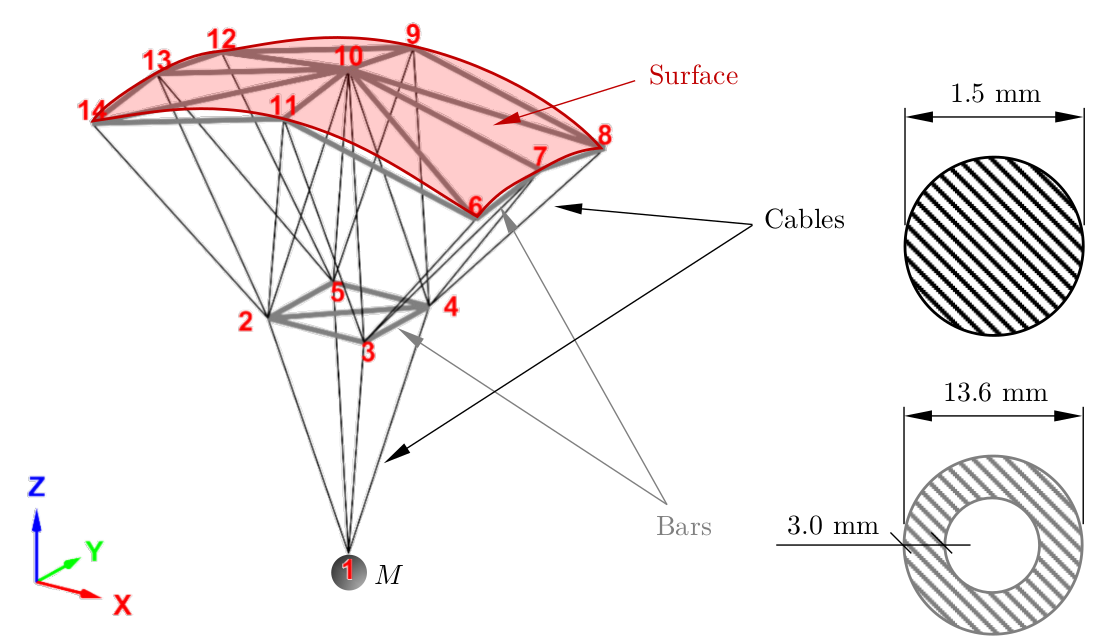
\includegraphics[width=0.8\textwidth]{img/parachute_definition.png}
	\caption{Definition of structure nodes and materials}
	\label{fig:definition}
\end{figure}

Materials properties of \textit{bars} and \textit{cables} are indicated in the
table \ref{tab:materials}

\begin{table}[h]
\centering
\begin{tabular}{|p{6cm}|c|c|}
\hline
\textbf{Property}  	& \textbf{Cables} & \textbf{Bars} \\ \hline
Density $(kg/m^3)$	& 1500		& 2300  \\ \hline
Young's Modulus (MPa)	& 200000	& 70000 \\ \hline
Yield strength (MPa)	& 300		& 240   \\ \hline
Section area $(mm^2)$	& 1.77		& 57.02 \\ \hline
\end{tabular}
\caption{Materials definition}
\label{tab:materials}
\end{table}



Reference \ref{fig:}\\
